\chapter{System Identification}    % For a new chapter (works in book and report class)
\subsubsection{Generalities}


Since experimental measurement procedure typically provides samples of input-output sequences, we start by considering identification of \textbf{\textit{discrete-time models}}. Procedure for identifying \textit{\textbf{continous-time models}} will be dicussed as well.\\
Here, we are dealling with \textbf{dynamical systems}. A system is called dynamic when its output at a given time is dependent on the all the inputs that have been inserted to the system up to that time, or equivalently we know the value of the input at the previous time-instance in and the initial value of the a set of variables called, \textbf{\textit{state variables}}.

The choice of state variables is not unique, but the number of them depend on the order of the system. It can be proved that \textbf{a possible choice for state variables is previous values of the output}.

It is assumed that, without loss of generality, any system, be linear or non-linear, can be modelled by means of the following \textit{\textbf{regression form}}:\\
\begin{equation}
y(k) = f(y(k-1), y(k-2), \cdots, y(k-n), u(k), u(k-1), \cdots, u(k-m), \theta_1, \theta_2, \cdots, \theta_{n+m+1})
\end{equation}
\begin{itemize}
\item \(n\) is the system order, \textbf{related to the number of state variables}
\item \(m < n\), always for the physical, or at any rate, causal systems.
\item \(u(k), y(k), k = 1, 2, ..., H\) are the \textbf{noise-free} samples of the input and output sequences, respectively.\\
\end{itemize}

\begin{center}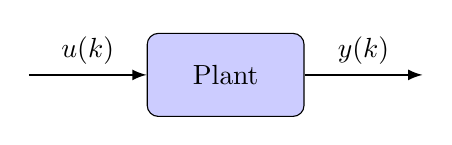
\begin{tikzpicture}[auto, node distance=2.5cm, >=latex]
    % Define styles
    \tikzstyle{block} = [rectangle, draw, fill=blue!20, 
                          text width=5em, text centered, rounded corners, minimum height=3em]
    \tikzstyle{input} = [coordinate]
    \tikzstyle{output} = [coordinate]
    \tikzstyle{arrow} = [thick,->,>=latex]
    
    % Nodes
    \node [input] (input) {};
    \node [block, right of=input] (plant) {Plant};
    \node [output, right of=plant] (output) {};
    
    % Draw arrows
    \draw [arrow] (input) -- node [above] {$u(k)$} (plant);
    \draw [arrow] (plant) -- node [above] {$y(k)$} (output);
\end{tikzpicture}\end{center}
\newpage

\subsubsection{General black-box EIV set-up}

\textit{Error-In-variables}, or EIV, problems refer to the most general case where both input and output collected samples are affected by noise, as represented in the figure \ref{fig:EIV}.\\
Two a-priori assumption is required at this point:\\
\begin{itemize}
\item a-priori assumption on the model: \(f \in F\) where \(F\) is a given class of functions
\item a-priori assumption on the noise: e.g. statistically distributed, or boundedness, etc
\end{itemize}
Then, we need to collect input-output data.
\begin{factbox}
\textbf{Without any assumption} about the noise corrupting the measurements, we cannot study the data at hand. Further, without any assumption about the structure, many structure can be find that map input samples to the output, that does not correspond to the behavior of the system. 
\end{factbox}

\begin{figure}[htbp]
    \centering
    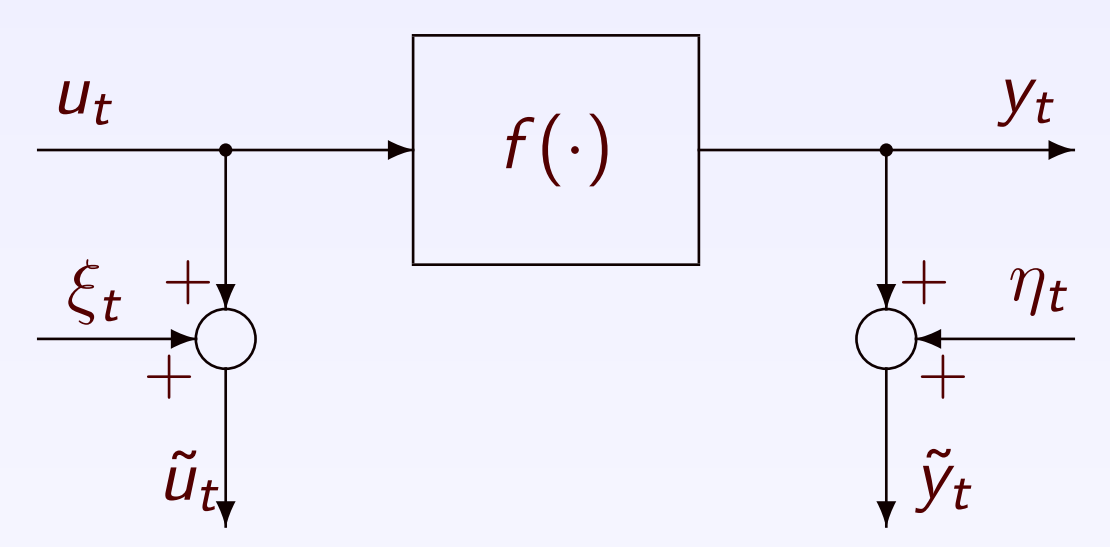
\includegraphics[width=0.5\textwidth]{images/EIV-problem.png}
    % Adjust width as needed
    \caption{a general shceme of error-in-variable problem}
    \label{fig:EIV}
\end{figure}

\subsubsection{A naive noiseless example}

Consider the following second order LTI discrete-time system (agent):

\begin{equation}
\begin{array}{l}
y(k) = f(y(k - 1), y(k - 2), u(k), u(k - 1), u(k - 2)) \\[1ex]
= -\theta_1 y(k - 1) - \theta_2 y(k - 2) + \theta_3 u(k) + \theta_4 u(k - 1) + \theta_5 u(k - 2)
\end{array}
\end{equation}

By introducing the backward shift operator \(q^{−r}\): \(q^{−r}(s(t))\)  = \(s(k − r)\), we can
rewrite the equation as:
\begin{equation}
y(k) = -\theta_1 q^{-1} y(k) - \theta_2 q^{-2} y(k) + \theta_3 u(k) + \theta_4 q^{-1} u(k) + \theta_5 q^{-2} u(k)
\end{equation}
Solving the equation in the \(y(k)\) we obtain:\\
\begin{equation}
y(k) = \frac{\theta_3 + \theta_4 q^{-1} + \theta_5 q^{-2}}{1 + \theta_1 q^{-1} + \theta_2 q^{-2}} u(k)
\end{equation}
By applying properties of the Z-transform it is possible to show that the system
transfer function G(z) can be obtained by simply replacing \(q^{-1}\) with \(z^{-1}\):
\begin{equation}
G(z) = \frac{Y(z)}{U(z)} = \frac{\theta_3 z^2 + \theta_4 z + \theta_5}{z^2 + \theta_1 z + \theta_2} u(k)
\end{equation}

Given H experimentally collected input-output samples matrix \ref{eq:regressor}, which is also called \textbf{\textit{regressor-matrix}}, leads to the following system of linear equations:
\begin{equation}
    y = A\theta
\end{equation}
where \(y = [y(3) y(4) ... y(H)]^T, \theta = [\theta_1 \theta_2 ... \theta_5]^T)\), and

\begin{equation}
    A = \left[
    \begin{matrix}
    -y(2) & -y(3) & u(3) & u(2) & u(1) \\
    -y(3) & -y(2) & u(4) & u(3) & u(2) \\
    \cdots & \cdots & \cdots & \cdots & \cdots   \\
    \cdots & \cdots & \cdots & \cdots & \cdots   \\
    -y(H-1) & -y(H-2) & u(H) & u(H-1) & u(H-2)
    \end{matrix} 
    \label{eq:regressor}
    \right]\\
\end{equation}

In this ideal, noise-free example, \(H = \text{the number of parameters} + \text{the order of the systerm}\), in this case, \(H = 7\) is enough to solve our 5-equations-and-5-unknown problem. The solution is going to be in the following form
:\\
\begin{equation}
    \theta = A^{-1} y
    \quad \overset{\text{Existence and Uniqueness Condition}}{\Rightarrow} \quad
    \begin{cases}
        
        A \in \mathbb{R}^{n \times n} \\
        \left|A\right| \neq 0
        
    \end{cases}
\end{equation}
One possible solution: apply to the system a random input sequence \(u\).\\

This formulation works for all the description that the output of the system is \textbf{linear with respect to the parameters}.

\begin{factbox}[Professor's Quote]
    In artificial-neural-network, the structure of \(f\) is different. Otherwise, the goal of any Machine Learning or System Identification problem is to find the mapping between the inputs and outputs.\\
    Regarding the importance of a-priori info about the system. The previous problem can also be solved for the following structure, that does no correspond to the behavior of a 2-order LTI system.
    \(y(k) = \theta_1 u(k) + \theta_2 u(k)^2 + \cdots + \theta_5 u(k)^5\)
\end{factbox}

\begin{example}[Example]
    It is desired to estimate the value of a resistor. A-priori info is that a resistor follows Ohm's law. As input signal, we insert current to our resistor and we measure the voltage across our resistor. \\
    
    \(y(k) = \theta u(k) \text{ s.th. y(.),u(.), }\theta \in \mathbb{R}\)\\
  
Here, \(\theta\) stands for the value of the resistor to be estimated. For this static system, which means the output of the system depends only on the values of the input at that time instance, we need a pair of noise-free input-output sample to estimate the value of the resistor. \\

\(\theta = \frac{y(1)}{u(1)}\)\\
\end{example}

\subsubsection{Noise effect}
If the measurements are corrupted by noise, the idea is to perform more measurements to average out the effect of the noise; \(H >> 2n + 1\) where n is the system order.\\

In this case, matrix\(A\) is not square anymore, which means it is not invertible. In this case, left pseudo-inverse, \((A^TA)^{-1}A^T\) of this matrix should be used.\\

\[
\tilde{y} = A \theta
\Rightarrow
A^T\tilde{y} = A^TA \theta
\Rightarrow
\theta = (A^TA)^{-1}A^T\tilde{y}
\]

This solution corresponids to the solution of the \textbf{\textit{Least Square}} problem.

\subsubsection{Least Square approach}

Least Square approach is solving the following optimization problem in order to find the parameters that minimizes a norm-2, or euclidian norm, cost-function.
\begin{equation}
    \hat{\theta_{LS}} = \arg \min \limits_{\theta} J(\theta) = \arg \min \limits_{\theta} \|\tilde{y} - A \theta\|_2
\end{equation}
In the context of system identification (but not only) θLS as what we refer to as
the Least square estimate of the system parameter vector. Computation burden of the Least square algorithms is quite low also for large H. The Least square estimate can be (also) computed recursively (i.e. online).
\newpage
\subsubsection{Consistency property of Least Square method}

If the following assumptions are satisfied:
\begin{enumerate}
\item The effect of the uncertainties corrupting the collected data can be taken into
account by introducing an additive term \textbf{e}, or equation error, as follows:
\[\tilde{y}(k) = y(k) + e(k)\]
\item  \(e(k)\), \(k = 1, 2, . . . , H\) are \textbf{independent and identically distributed} (iid) random
variables; typically it is assumed that \(e\) can be modeled as a white, zero-mean
Gaussian noise.
\end{enumerate}
Least-Square method enjoys the following interesting property:
\begin{equation}
\lim\limits_{H \to \infty} E[\theta_{LS}] = \theta
\end{equation}
Pay attention that, in our assuption, there is no argument about the variance of the noise. This is the reason why \textit{LS} method is so appealing in practice. Nevertheless, if these two assumtions does not hold, this method is not going to provide suitable results.

\begin{QandAbox}
\textbf{This property of the Least Square solution holds only when the afforementioned consistency conditions hold.\\
Every time, this method is to be applied to an engineering problem, these two assumptions should be satisfied so that the concistency property holds.
}\end{QandAbox} \vspace{0.5cm}

\textbf{As to the first assumption}, Let's check whether such an assuption is satisfied when we collect the data by performing a real experiment in its most general form, Error-In-Variable form \ref{fig:EIV}. Considering a second-order LTI system - a-priori information about the system - we have:
\[
y(k) = -\theta_1 y(k - 1) - \theta_2 y(k - 2) + \theta_3 u(k) + \theta_4 u(k - 1) + \theta_5 u(k - 2)
\]
Additionally, considering EIV form:
\[
\begin{cases}
    \tilde{y}(k) = y(k) + \eta(k)\\
    \tilde{u}(k) = u(k) + \zeta(k)
\end{cases}
\]

\begin{factbox}[Regarding the noise]
It's correct that the same sensor might be used for obtaining data samples - suggensting that the noises are dependent. Nonetheless, we assume that all the systematic error of the sensor is taken into considerations, and \textbf{\(\zeta(.)\) and \(\eta(.)\) are undeterministic noises}.\\

Also, here, an \textbf{absolute error} is considered which is the form:\\
\(\tilde{y}(.) = y(.) + \eta(.)\)
\end{factbox}
\newpage
\begin{factbox}
In case of \textbf{relative error}, the following manipulations may be done which leads to a mathematically equivalent structure.\\
\(\tilde{y}(.) = y(.)(1 + \eta(.))\)\\
Also in this case, the same result is going to be obtained.
\end{factbox}
By replacing \(y(k)\) and \(u(k)\) in the difference equation of the system the following is obtained:
\[
\begin{array}{l}
\tilde{y}(k) - \eta(k) = -\theta_1(\tilde{y}(k-1)) - \eta(k-1) -\theta_2(\tilde{y}(k-2) - \eta(k-2)) + \theta_3(\tilde{u}(k) + \xi(k)) \\[1ex] 
+ \theta_4(\tilde{u}(k-1) + \xi(k-1))
 \theta_5(\tilde{u}(k-2) + \xi(k-2)) \\[1ex] 
\Rightarrow \\[1ex]
\tilde{y}(k)= -\theta_1 \tilde{y}(k - 1) - \theta_2 \tilde{y}(k - 2) + \theta_3 \tilde{u}(k) + \theta_4 \tilde{u}(k - 1) + \theta_5 \tilde{u}(k - 2) \\[1ex]
\textcolor{red}{\fbox{\textcolor{black}{$+ \theta_1\eta(k-1) + \theta_2\eta(k-2) - \theta_3\xi(k) - \theta_4\xi(k-1) - \theta_5\xi(k-2) + \eta(k) $}}} =: + e(k) \\
\end{array}
\]
Hence:
\begin{equation}
\begin{array}{l}
\tilde{y}(k)= -\theta_1 \tilde{y}(k - 1) - \theta_2 \tilde{y}(k - 2) + \theta_3 \tilde{u}(k) + \theta_4 \tilde{u}(k - 1) + \theta_5 \tilde{u}(k - 2) + \textbf{e(k)}
\end{array}
\end{equation}

As it can be seen, considering the afformentioned assumption about noise and system, \textbf{the first assumption of the concistency property is hold!}.\\

\textbf{As to the second assumption}, it is needed to check whether the sequence \(e(k)\), \(k = 1,2, \cdots, H\) is i.i.d, independent and identically distributed. To do so, the value of \(e(k)\) is written for two time instances \(k\) and \(k+1\):
\[
\begin{array}{l}
e(k) = \theta_1\eta(k-1) + \theta_2\eta(k-2) - \theta_3\tilde{u}(k) - \theta_4\tilde{u}(k-1) - \theta_5\tilde{u}(k-2) \\[1ex]
e(k+1) = \theta_1\eta(k) + \theta_2\eta(k-1) - \theta_3\tilde{u}(k+1) - \theta_4\tilde{u}(k) - \theta_5\tilde{u}(k-1)
\end{array}
\]
As it can be seen, since both \(e(k+1)\) and \(e(k)\) depend on common variables, the sequence \(e(.)\) is not i.i.d; \textbf{the second is not satisfied}.\\

In conclusion, Least-Square estimation applied to \(\tilde{u}(.)\) and \(\tilde{y}(.)\), collected from an experiment enjoying the EIV structure provide and estimation, \(\hat{theta}_{LS}\) which does not enjoy consistency property. That is,
\[
\lim\limits_{H \to \infty} E[\theta_{LS}] \neq \theta
\]

\textbf{Results:}\\
Least-Square estimation \textbf{DOES NOT} enjoy the consistency properties when applied to input-output data obtained by performing an experiment on a dynamicsl system in the presence of an uncertainty entering the problem according to the \textit{EIV} or \textit{Output-Error} setting. 
\newpage
In which cases, assuption 1 and 2 are both satisfied?\vspace{0.5cm} \\
\(
\begin{cases}
\text{Assuption 1:}\\ 
\hspace{1cm}
\begin{array}{l}
\tilde{y}(k)= -\theta_1 \tilde{y}(k - 1) - \theta_2 \tilde{y}(k - 2) - \cdots -\tilde{y}(k - n) \\[1ex] + \theta_{n+1} \tilde{u}(k) + \theta_{n+2} \tilde{u}(k - 1) + \cdots + \theta_{n+m+1}\tilde{u}(k - m) + \textbf{e(k)}
\end{array}\\
\text{Assumption 2:}\\
\hspace{1cm}
e(.) \text{ is an i.i.d variable}
\end{cases}
\)\\

Let's consider, for the sacke of simplicity and without loss of generality, that the inputs are perfectly known.
\[
\begin{array}{l}
\tilde{u}(.) = u(.) \\ [2ex]
\tilde{y}(k)= -\theta_1 \tilde{y}(k - 1) - \theta_2 \tilde{y}(k - 2) - \cdots -\tilde{y}(k - n) \\[1ex] + \theta_{n+1} u(k) + \theta_{n+2} u(k - 1) + \cdots + \theta_{n+m+1} u(k - m) + e(k) \\[2ex]
\Rightarrow \\[2ex]
\tilde{y}\left[\theta_{n+1} + \theta_{n+2} q^{-1} + \cdots + \theta_{n+m+1} q^{-m}\right] =
= u(k)\left[1 + \theta_1 q^{-1} + \theta_2 q^{-2} + \cdots + \theta_n q^{-n}\right] + e(k)\\[2ex]
\Rightarrow \\[2ex]
\tilde{y}
= \frac{\left[1 + \theta_1 q^{-1} + \theta_2 q^{-2} + \cdots + \theta_n q^{-n}\right]}{\left[\theta_{n+1} + \theta_{n+2} q^{-1} + \cdots + \theta_{n+m+1} q^{-m}\right]}u(k) 
+ \frac{1}{\left[\theta_{n+1} + \theta_{n+2} q^{-1} + \cdots + \theta_{n+m+1} q^{-m}\right]}e(k)
\end{array}
\]
Now, considering that the equivalent of delay-operator in the \(z\)-domain is \(z\):
\[
\tilde{y} = G(z) u(z) + \frac{1}{D(z)} e(z)
\]
where,
\[
G(z) = \frac{N(z)}{D(z)} 
\begin{cases}
N(z) = \left[1 + \theta_1 q^{-1} + \theta_2 q^{-2} + \cdots + \theta_n q^{-n}\right] \\
D(z) = \left[\theta_{n+1} + \theta_{n+2} q^{-1} + \cdots + \theta_{n+m+1} q^{-m}\right]
\end{cases}
\]
The block diagram scheme of the abovementioned equation is drawn hereunder.\\
\begin{center}
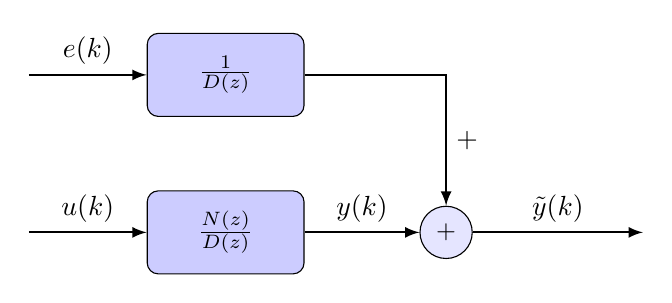
\begin{tikzpicture}[auto, node distance=2.5cm, >=latex]
    % Define styles
    \tikzstyle{block} = [rectangle, draw, fill=blue!20, 
                          text width=5em, text centered, rounded corners, minimum height=3em]
    \tikzstyle{input} = [coordinate]
    \tikzstyle{output} = [coordinate]
    \tikzstyle{sum} = [draw, fill=blue!10, circle, node distance=1.5cm]
    \tikzstyle{arrow} = [thick,->,>=latex]
    
    % Nodes
    \node [input] (input) {};
    \node [block, right of=input] (Gz) {$\frac{N(z)}{D(z)}$};
    \node [output, right of=Gz] (output) {};
    \node [block, above of=Gz, node distance=2cm] (Dz) {$\frac{1}{D(z)}$};
    \node [sum, right of=Gz, node distance=2.8cm] (sum) {\small$+$};
    \node [input, left of=Dz, node distance=2.5cm] (errorInput) {};
    \node [output, right of=sum, node distance=2.5cm] (ytilde) {};

    % Draw arrows
    \draw [arrow] (input) -- node [above] {$u(k)$} (Gz);
    \draw [arrow] (Gz) -- node [above] {$y(k)$} (sum);
    \draw [arrow] (sum) -- node [above] {$\tilde{y}(k)$} (ytilde);
    
    % Error signal and Dz block
    \draw [arrow] (errorInput) -- node [above] {$e(k)$} (Dz);
    \draw [arrow] (Dz) -| node [near end, right] {$+$} (sum);

\end{tikzpicture}
\end{center}



LS estimation is going to make sense, if and only if the sensor used for collecting data affect the collected data with a measurement noise obtained as a random, white signal \(e(k)\) that is filtered by the denominator of the system to be identified, \textbf{which does not make sense}!!!; the name of this setting is \textbf{\textit{Error-in-Equation}} setting, which does not correspond to data collection in practical situation, since the sensor does not know how to filter the noise to obtain \(e(k)\) that are probabilistically independent.\\

Our general conclusion is that Least-Square estimation should not be used when our collected via \textbf{a real experiment, EIV setting or OE setting}(OE is a subset of EIV problem, meaning that the input signal is perfectly known and the uncertainty affects output measurements dirrectly); that is, when we collect data from the experiment, even if the input is perfectly known, the output would be corrupted by additive or multiplicative noise by the data; using these data samples, LS method does not enjoy consistency property. However, Assumption 1 is satisfied and perfectly make sense when the LTI system to be identified is such that \(D(z) =  1\).\\
\[
D(z) = 1 \Rightarrow
\begin{cases}
\textcolor{red}{\fbox{\textcolor{black}{$
\text{Identification of \textbf{FIR (finite impulse response)}}
$}}}\\
\textcolor{red}{\fbox{\textcolor{black}{$\text{Identification of \textbf{static systems}}
$}}}
\end{cases}
\]
The reason is that when \(D(z) = 1\), the equation error \(e(k)\) is actually playing the role of the output measurement error \(\eta(k)\), which means i.i.d by definition, thereby satisfying also assumption 2. Now, some identification problems where both assumptions are satisfied.\\

\begin{example}[Examples that satisfies assuptions of the consistency property]
\textbf{1) A Finite-Pulse Response system} is defined in the following fashion:\\
    \(\mathbb{S}: y(k) = \theta_1 u(k) + \theta_2 u(k-1) + \cdots + \theta_n u(k-n+1)\)\\
  
Measured samples of the output have the following form:\\
\(
\begin{array}{l}
\tilde{y}(k) = y(k) + \eta(k)\\
\Rightarrow\\
\tilde{y} = \theta_1 u(k) + \theta_2 u(k-1) + \cdots + \theta_n u(k-n+1) + e(k)
\end{array}
\)\\
Where \(e(.) = \eta(.) \).\\

\textbf{2) Static Systems}: \\
\(\mathbb{S}: y(k) = f(u(k),\theta) = \theta_1 f_1(u(k)) + \theta_2 f_2(u(k)) + \cdots + \theta_n f_n(u(k))\)\\
Measured samples of the output have the following form:\\
\(
\begin{array}{l}
\tilde{y}(k) = y(k) + \eta(k)\\
\Rightarrow\\
\tilde{y} = \theta_1 f_1(u(k)) + \theta_2 f_2(u(k)) + \cdots + \theta_n f_n(u(k)) + e(k)
\end{array}
\)\\
such basis functions as polinomials or sinusoidal functions.\\
Where again, \(e(.) = \eta(.) \).\\
\end{example}
\begin{example}
Examples of functions \(f_n\) can be any set of 
In this case, the error \(e(k)\) enters the equation in an \textit{Error-in-Equation} fashion, which is required to satisfy the second assumption of the consistency property of LS.

\begin{center}
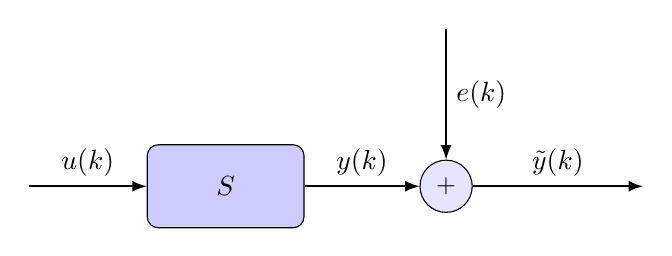
\begin{tikzpicture}[auto, node distance=2.5cm, >=latex]
    % Define styles
    \tikzstyle{block} = [rectangle, draw, fill=blue!20, 
                          text width=5em, text centered, rounded corners, minimum height=3em]
    \tikzstyle{input} = [coordinate]
    \tikzstyle{output} = [coordinate]
    \tikzstyle{sum} = [draw, fill=blue!10, circle, node distance=1.5cm]
    \tikzstyle{arrow} = [thick,->,>=latex]
    
    % Nodes
    \node [input] (input) {};
    \node [block, right of=input] (Gz) {$\mathbb{S}$};
    \node [output, right of=Gz] (output) {};
    \node [sum, right of=Gz, node distance=2.8cm] (sum) {\small$+$};
    \node [input, above of=sum, node distance=2cm] (errorInput) {};
    \node [output, right of=sum, node distance=2.5cm] (ytilde) {};

    % Draw arrows
    \draw [arrow] (input) -- node [above] {$u(k)$} (Gz);
    \draw [arrow] (Gz) -- node [above] {$y(k)$} (sum);
    \draw [arrow] (sum) -- node [above] {$\tilde{y}(k)$} (ytilde);
    
    % Error signal directly to summation point
    \draw [arrow] (errorInput) -- node [right] {$e(k)$} (sum);
\end{tikzpicture}
\end{center}
In these cases, both assumptions are satisfied, since, by assumption \(\eta\) is considered to be i.i.d, and since the error directly enters the output the first assumption is satisfied, which means:\\
\(\lim\limits_{H \to \infty} \hat{\theta}_{LS} = \theta\)\\
\end{example}

what is critical is the combination of the two assumptions, and no matter what is the structure of the system, we can always manage to define \(e(k)\) in a way that it satisfies the first assumption. The problem is that we also have to impose an additional condition, being i.i.d, on \(e(k)\) so that also the second assumption is satisfied, while based on the system equation and the way we defined \(e(k)\), this condition might not be satisfied.\\

Our next step is to reformulate this problem in a different fashion, by modifying assumption 2. In another words, it is aimed to replace assumption 2 by a "weaker assumption." This change of perspective leads to what we call \textit{Set-membership} approach to system identification.\\

\begin{QandAbox}[What about the unreachable and unobservable modes of the system?]
This is a somehow phylosophical question, which can be answered in two way:
\begin{enumerate}
\item From the practical point of view, at most engineering cases, the system that is designed does not include unobservable modes that are unstable. 
\item From a phylosophical point of view, these modes cannot be identified through input-output data collection.
\end{enumerate}
\end{QandAbox}

